\documentclass[lecture.tex]{subfiles}

\begin{document}

\exercice{Jessy Lefeuve}
%\video{https://youtu.be/blablabla}
\enonce{rdm-0026}{Etude du bras de la sonde Osiris-Rex}

Le 21 octobre dernier, la sonde Osiris-Rex (figure \ref{figA}) est entrée en contact avec l’astéroïde Bennu, avec pour objectif de rapporter des échantillons de matière de cet astéroïde sur Terre. Pour récupérer ces échantillons de matière, la sonde est équipée d’un bras dont nous nous proposons ici l’étude.

\begin{figure}[h!]
  \centering
  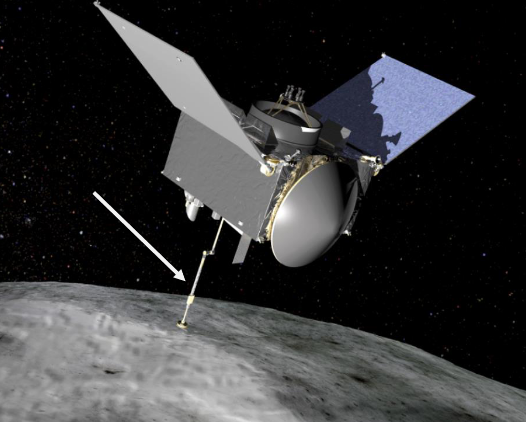
\includegraphics[scale=0.4]{figA0026.png}
  \caption{Sonde spatiale Osiris-Rex à l’approche de l’astéroïde Bennu}
  \label{figA}
\end{figure}

En première approximation, nous négligerons les effets dynamiques et considérerons donc un problème statique. Le bras (montré par la flèche sur la figure \ref{figA}) sera modélisé
par une poutre encastrée à une extrémité comme le présente le schéma suivant.

\begin{center}
  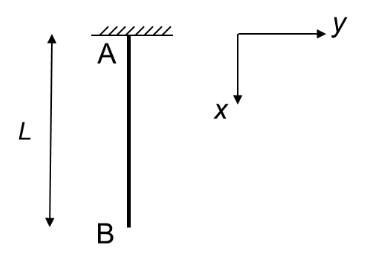
\includegraphics[scale=0.4]{figB0026.png}
\end{center}

\bigskip

\begin{description}

  \item[Première partie : Charge idéale] \ \par
  %
  Dans une configuration idéale, le bras est amené à entrer en contact de façon normale au sol. L’impact est modélisé par l’effort $F_{imp}$ orienté selon l’axe $-x$ (problème plan) sur le schéma suivant.
  \begin{center}
    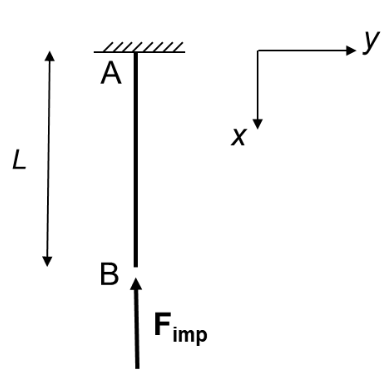
\includegraphics[scale=0.4]{figC0026.png}
  \end{center}
  %
  \begin{enumerate}
    \item Démontrez l'isostaticité de la structure.
    \item Déterminez les expressions des inconnues de liaisons par application du Principe Fondamental de la Statique (PFS).
    \item Déterminez les expressions des efforts internes à la structure $N$, $T$ et $M$ en fonction de l'abscisse $x$ dans le cas de cette charge idéale. Tracer les diagrammes des efforts internes.
    \item Quel phénomène physique peut apparaître dans le cas de cette sollicitation de compression spécifiquement ?
  \end{enumerate}

  \item[Deuxième partie : Charge réelle] \ \par
  %
  L’impact se faisant sur un sol non orthogonal à l’axe de la poutre, la sollicitation réelle $F_{imp}$ est orientée selon l’axe $-x$ et l’axe $+y$ (problème plan) comme sur le schéma suivant.
  \begin{center}
    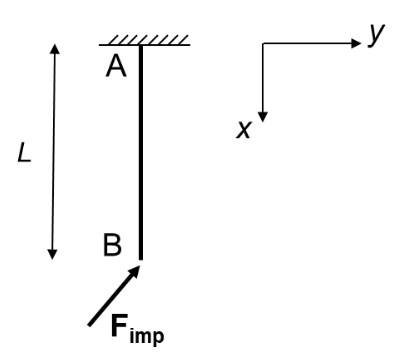
\includegraphics[scale=0.4]{figD0026.png}
  \end{center}
  %
  \begin{enumerate}
    \item En projetant $F_{imp}$ sur les axes $x$ et $y$ (projections notées respectivement $F_{impx}$ et $F_{impy}$, déterminez les expressions des nouvelles inconnues de liaisons.
    \item Déterminez les expressions des efforts internes à la structure $N$, $T$ et $M$ en fonction de l'abscisse $x$ pour cette nouvelle sollicitation.
    \item Tracer les diagrammes des efforts internes à la structure $N$, $T$ et $M$ en fonction de l'abscisse $x$ pour cette sollicitation réelle.
  \end{enumerate}

\end{description}

\finenonce{rdm-0026}
\finexercice


\end{document}
